% requirements:
%	TeX environments: TeXlive/MacTeX or MiKTeX
%	compiler: XeLaTeX
%
% ---------------------------------------------------------------------------- %
%                                   preamble                                   %
% ---------------------------------------------------------------------------- %
\documentclass[a4paper]{article}
% 10.5pt = 5 hao

% ---------------------------------- layout ---------------------------------- %
\usepackage[a4paper,top=2.5cm,bottom=2.5cm,left=3cm,right=3cm,% margins
			headheight=1.5cm,headsep=1.5em,
			footskip=2em,
			]{geometry}

% ------------------------------- math symbols ------------------------------- %
% 载入常用的数学包, 符号包
\usepackage{amsmath}
\usepackage{amsfonts}
\usepackage{amssymb}
\usepackage{mathrsfs}
\usepackage{blindtext}

%----------------------------------------------------------------%
%% linespace 行间距,段间距等等
\usepackage{setspace}
% \usepackage{indentfirst} % then the first line of each title should start with a indent.
% 定义标题和段落样式
% 定义1.5倍行距
\renewcommand{\baselinestretch}{1.62}
\setlength{\baselineskip}{12pt}   % set the fixed value of the lineskip
\setlength\parskip{\baselineskip} % set the space between the paragraphs, set the variable \parskip \baselineskip
% parindent
\setlength{\parindent}{0pt}

%----------------------------------------------------------------%
% fonts (style, color, size). 字体的大小,颜色,以及定义常用的字号
\usepackage{ctex}		 	% If you are lazy, the CTEX suit is enough.
% Chinese font
\usepackage{xeCJK}		 	% For the Chinese through XeLaTex
\setCJKmainfont{SimSun} 	% set the mainfont of Chinese as songti. (serif) for
\setCJKsansfont{SimSun} 	% sans serif font for \textsf
\setCJKmonofont{SimSun} 	% monospace font for \texttt
% \punctstyle{kaiming}  	% Remove the space used by symbols like comma. Special for the mainland students like us HUSTers.
\setCJKfamilyfont{song}{SimSun}                       % 宋体 song
\newcommand{\song}{\CJKfamily{song}}
\setCJKfamilyfont{kai}{KaiTi}                         % 楷体  kai
\newcommand{\kai}{\CJKfamily{kai}}
\setCJKfamilyfont{hwzs}{STZhongsong}                  % 华文中宋  hwzs
\newcommand{\hwzs}{\CJKfamily{hwzs}}
\setCJKfamilyfont{hei}{SimHei}                        % 黑体  hei
\newcommand{\hei}{\CJKfamily{hei}}
% English font
\usepackage{fontspec}% Then you can use the fonts installed at your device.
\setmainfont{Times New Roman}
\setsansfont{Times New Roman}
\setmonofont{Times New Roman}
%\setsansfont{[foo.ttf]} % for the fonts at this default path.
% font Color 利用definecolor自己可以定义颜色
\usepackage{xcolor}
\definecolor{MSBlue}{rgb}{.204,.353,.541}
\definecolor{MSLightBlue}{rgb}{.31,.506,.741}
% font Size (I use pinyin represents the corresponding size in Microsorft Word)
% \newcommand{\chuhao}{\fontsize{42pt}{\baselineskip}\selectfont}
\newcommand{\xiaochuhao}{\fontsize{36pt}{\baselineskip}\selectfont}
% \newcommand{\yihao}{\fontsize{28pt}{\baselineskip}\selectfont}
\newcommand{\erhao}{\fontsize{21pt}{\baselineskip}\selectfont}
\newcommand{\xiaoerhao}{\fontsize{18pt}{\baselineskip}\selectfont}
\newcommand{\sanhao}{\fontsize{15.75pt}{\baselineskip}\selectfont}
\newcommand{\sihao}{\fontsize{14pt}{18pt}\selectfont}
\newcommand{\xiaosihao}{\fontsize{12pt}{18pt}\selectfont}
\newcommand{\wuhao}{\fontsize{10.5pt}{18pt}\selectfont}
% \newcommand{\xiaowuhao}{\fontsize{9pt}{\baselineskip}\selectfont}
% \newcommand{\liuhao}{\fontsize{7.875pt}{\baselineskip}\selectfont}
% \newcommand{\qihao}{\fontsize{5.25pt}{\baselineskip}\selectfont}


% ---------------------------------------------------------------------------- %
%% header and footer 页眉,页脚
\usepackage{fancyhdr} % for header and footer

% 设置页眉样式
\newcommand{\headstyle}{
 \fancyhead[C]{ \hwzs\wuhao 华\hspace{0.5em}中\hspace{0.5em}科\hspace{0.5em}技\hspace{0.5em}大\hspace{0.5em}学\hspace{0.5em}课\hspace{0.5em}程\hspace{0.5em}设\hspace{0.5em}计\hspace{0.5em}(报\hspace{0.5em}告)}
}

% 设置页脚样式
\newcommand{\footstyle}{\fancyfoot[C]{\wuhao\thepage}
 \fancyfoot[L]{\rule[5pt]{6.7cm}{0.4pt}}
 \fancyfoot[R]{\rule[5pt]{6.7cm}{0.4pt}}
}
\pagestyle{fancy}
\fancyhf{} % 清空原有样式
\headstyle
\footstyle
% 定义一种新的格式叫做main
\fancypagestyle{main}{%
 \fancyhf{} % 清空原有样式
 \headstyle
 \footstyle
}
\renewcommand{\headrulewidth}{0.4pt}
% \renewcommand{\footrulewidth}{0.4pt}
% \renewcommand{\headrule}{\rule{\textwidth}{0.4pt}}

% ---------------------------------------------------------------------------- %
% set the styles of sections at all levels
% 设置各个标题样式
% 不需要使用part和chapter层级
\usepackage{titlesec}
\usepackage{titletoc}
\titleformat{\section}{\centering\hei\bfseries\xiaoerhao}{\thesection}{1em}{} % 在section标题编号后面加个点
% \titlelabel{\thetitle.\quad} % add a dot after the counter for all levels of sections
% \titleformat*{\section}{\wuhao\bfseries} % 设置标签的形式,5号加粗
\titleformat*{\subsection}{\raggedright\hei\bfseries\sihao}
\titleformat*{\subsubsection}{\raggedright\hei\bfseries\xiaosihao}
\titleformat{\paragraph}[hang]{\raggedright\hei\bfseries\xiaosihao}{\theparagraph}{1em}{}[]

% manual
% \titleformat{command}[shape]{format}{label}{sep}{before-code}[after-code]
% \titlespacing{command}{left}{before-sep}{after-sep}
% 设置新的层级subsubsubsection
\setcounter{tocdepth}{4}
\setcounter{secnumdepth}{4}

% \newcommand{\sectionbreak}{\clearpage} % 小节从新的一页开始
% 根据学校要求设置新的section, subsection, subsection,  paragraph

% set the content of section and so on
\newcommand\seccontent{
	\song
	\xiaosihao % 默认五号字体, 行间距为1.5*\baselineskip
    \setlength{\parindent}{2em} % 首段缩进两个M字符
    \setlength{\parskip}{0pt}
    }
\newcommand\tabcontent{
	\song
	\wuhao % 默认五号字体, 行间距为1.5*\baselineskip
	\setlength{\parindent}{2em} % 首段缩进两个M字符
	\setlength{\parskip}{0pt}
}


% ---------------------------------------------------------------------------- %
% for the style of theorems, definitions, proofs and remarks 定义数学里面一些常用的环境
\usepackage{amsthm}
\newtheorem{thm}{\textbf{定理}}[section]
% The section in [] can be replaced by chapter or subsection
\theoremstyle{definition} 
\theoremstyle{plain}
\theoremstyle{remark}

% ---------------------------------------------------------------------------- %
% for the caption and reference 图表及公式的编号规范
\usepackage{float} 		 		  	% table figure positioning
\usepackage{caption}
\captionsetup[figure]{labelformat=default, labelsep=quad,name={图}}
\captionsetup[table]{labelformat=default,labelsep=quad,name={表}}
% 设置图表标题的计数方式
\renewcommand{\thefigure}{\ifnum \thesection>0 \thesection-\fi \arabic{figure}} % set caption label style to 2-1
\renewcommand{\thetable}{\ifnum \thesection>0 \thesection-\fi \arabic{table}} % set caption label style to 2-1
\DeclareCaptionFont{mylabelfont}{\hei\xiaosihao}
\captionsetup[figure]{font=mylabelfont}
\captionsetup[table]{font=mylabelfont}

% 设置图表的autoref的格式
\newcommand{\reffig}[1]{图 \ref{#1}}
\newcommand{\reftab}[1]{表 \ref{#1}}
% 公式的编号格式
\renewcommand\theequation{\arabic{section}-\arabic{equation}}


\usepackage{graphicx} % To include graphixs 添加图所需的包

\graphicspath{{./graphics/}} %设置图片路径
\usepackage{booktabs} % To create three line table including the commands toprule, bottomrule, and midrule
% \usepackage{colortbl} %
% 使用tabularx库并定义新的左右中格式
\usepackage{tabularx}
\usepackage{makecell}
\newcolumntype{L}{X}
\newcolumntype{C}{>{\centering \arraybackslash}X}
\newcolumntype{R}{>{\raggedright \arraybackslash}X}

% ---------------------------------------------------------------------------- %
% set the style of counters 设置计数器
% 设置重新计数的位置
\makeatletter
\@addtoreset{footnote}{page}
\@addtoreset{figure}{section}
\@addtoreset{table}{section}
\@addtoreset{equation}{section}
\makeatother

% ---------------------------------------------------------------------------- %
% tableofcontents, listoftables and listoffigures 目录
%\renewcommand\listfigurename{插图列表}
%\renewcommand\listtablename{表格列表}
%\titlecontents{标题名}[左间距]{标题格式}{标题标志}{无序号标题}{指引线与页码}[下间距]
%\dottedcontents{section}[2.55em]{\song \xiaosihao \bfseries}{2.5em}{1em}
\usepackage{tocloft}
\renewcommand{\contentsname}{\centerline{ \hei\bfseries\xiaoerhao 目\hspace{2em}录}}
\titlecontents{section}[3em]{\song\xiaosihao\bfseries}{\contentslabel{3em}}{\hspace*{-3em}}{\normalfont\titlerule*[8pt]{.}\contentspage}
\titlecontents{subsection}[3em]{\song\xiaosihao}{\contentslabel{3em}}{\hspace*{-3em}}{\titlerule*[8pt]{.}\contentspage}
\titlecontents{subsubsection}[4em]{\song\xiaosihao}{\contentslabel{4em}}{\hspace*{-4em}}{\titlerule*[8pt]{.}\contentspage}
\titlecontents{paragraph}[5em]{\song\xiaosihao}{\contentslabel{5em}}{\hspace*{-5em}}{\titlerule*[8pt]{.}\contentspage}


% ---------------------------------------------------------------------------- %
% 设置声明页
% 使用特殊符号
\usepackage{amssymb}
\usepackage{wasysym}


% ---------------------------------------------------------------------------- %
%	---	定义列表项,列举的样式
\usepackage{enumitem}
\setlist{noitemsep}

% ---------------------------------------------------------------------------- %
% \usepackage{makeindex} For the index 索引
\usepackage{listings} % For the code. 代码

% ---------------------------------------------------------------------------- %
% 设置脚注

% ---------------------------------------------------------------------------- %
%% For the hyperlink and bookmark 超链接及书签,(这样生成的pdf中的引用直接点击链接即可到达目的地)

\usepackage[bookmarks=true,colorlinks,linkcolor=black,citecolor=black,urlcolor=purple]{hyperref}% 设置超链接并修改风格

% ---------------------------------------------------------------------------- %
%% For the appendix, 附录
% 设置附录
\usepackage{appendix}
\renewcommand{\appendixname}{附录}

% ---------------------------------------------------------------------------- %
% for the titlepage 标题页,此处可以省略,建议直接使用官方给出的标题页即可
\usepackage{titling}
% 重置命令 maketitle
\renewcommand{\maketitle}{
	\def\HUSTtitlelength{12em}
 	\begin{titlepage}
		\begin{center}
			\vspace*{0em}
			
\includegraphics[height=1.61cm]{HUSTlogo.eps}\\
%
			\vspace*{4em}
%
			{\xiaochuhao \hwzs \bfseries 电子线路实验报告}\\
%
			\vspace*{6em}
			{\erhao \hei \bfseries \thetitle}

			\vspace*{6em}
			{\sanhao \hwzs
				\renewcommand\arraystretch{2.7}
				\begin{tabular}{lc}
					\makebox[4em][s]{院 \hfill 系} &
					\underline{\makebox[\HUSTtitlelength]{\school}} \\
					\makebox[4em][s]{专业班级} &
					\underline{\makebox[\HUSTtitlelength]{\classnum}} \\
					\makebox[4em][s]{姓 \hfill 名} &
					\underline{\makebox[\HUSTtitlelength]{\theauthor}} \\
					\makebox[4em][s]{学 \hfill 号} &
					\underline{\makebox[\HUSTtitlelength]{\stunum}} \\
					\makebox[4em][s]{指导教师} &
					\underline{\makebox[\HUSTtitlelength]{\instructor}} \\
			  \end{tabular}
		    }

			\vspace{4em}
			{\sanhao \hwzs \thedate}

		\end{center}
	\end{titlepage}
}

\usepackage{multirow}

% ------------------------------------ 标题页 ----------------------------------- %
\title{实验一:集成运算放大器的基本应用} % 论文题目
\def\school{电子信息与通信学院} % 院系
\def\classnum{信卓2201班} % 专业班级
\author{董浩} % 姓名
\def\stunum{U202213781}	% 学号
\def\instructor{陈林} % 指导老师
\date{\today} % 日期


% ---------------------------------------------------------------------------- %
%                                   document                                   %
% ---------------------------------------------------------------------------- %
\begin{document}

\maketitle


\tableofcontents
\thispagestyle{main}

\clearpage
\setcounter{page}{1}
\renewcommand{\thepage}{\arabic{page}}

% ----------------------------------- 主体内容 ----------------------------------- %
\seccontent

\section{实验目的}
\begin{enumerate}
	\item 熟练掌握集成运算放大器的正确使用方法。
	\item 掌握用集成运算放大器构成各种基本运算电路的方法。
	\item 学会合理选用示波器的直流、交流耦合方式观察不同波形的方法。
\end{enumerate}
\section{实验元器件}


\begin{table}[H]
	\centering
	\large
	\begin{tabular}{|c|c|c|}
		\hline
		名称                  & 型号(参数) & 数量 \\ \hline
		集成运算放大器             & NE5532 & 1  \\ \hline
		\multirow{6}{*}{电阻} & 100Ω   & 1  \\ \cline{2-3}
		                    & 500Ω   & 1  \\ \cline{2-3}
		                    & 1KΩ    & 2  \\ \cline{2-3}
		                    & 5.1KΩ  & 1  \\ \cline{2-3}
		                    & 10KΩ   & 1  \\ \cline{2-3}
		                    & 100KΩ  & 1  \\ \hline
		电容                  & 0.22μF & 1  \\ \hline
	\end{tabular}
	\caption{实验元器件表格}
	\label{实验元器件表格}
\end{table}

\clearpage

\section{实验任务}
\subsection{研究电压跟随器的作用}

(1)按\reffig{直接连接}连接电路。
断开开关K。输入$f=1 \mathrm{kHz},V_{ipp}=1 \mathrm{V}$的正弦信号,用示波器观察输出波形。

闭合开关K。观察输出波形的变化情况。
分别记录K闭合前、后信号源输出信号的峰-峰值,计算信号源的内阻Rs,并解释100Ω负载电阻连接到信号源上产生的负载效应。


(2) 按\reffig{通过电压跟随器连接}连接电路。
仍然从信号源送出频率为1kHz、峰峰值为1V的正弦信号,用示波器观察输入、输出波形(幅值与相位关系)。分别记录接上$\mathrm{R_L}$和去掉$\mathrm{R_L}$,两种情况下输出信号$\mathrm{v_o}$的大小,并解释观察到的实验现象。


\begin{figure}[H]
	\begin{minipage}[t]{0.5\linewidth}
		\centering
		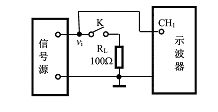
\includegraphics[width=1\textwidth]{直接连接}
		\caption{直接连接}
		\label{直接连接}
	\end{minipage}%
	\begin{minipage}[t]{0.5\linewidth}
		\centering
		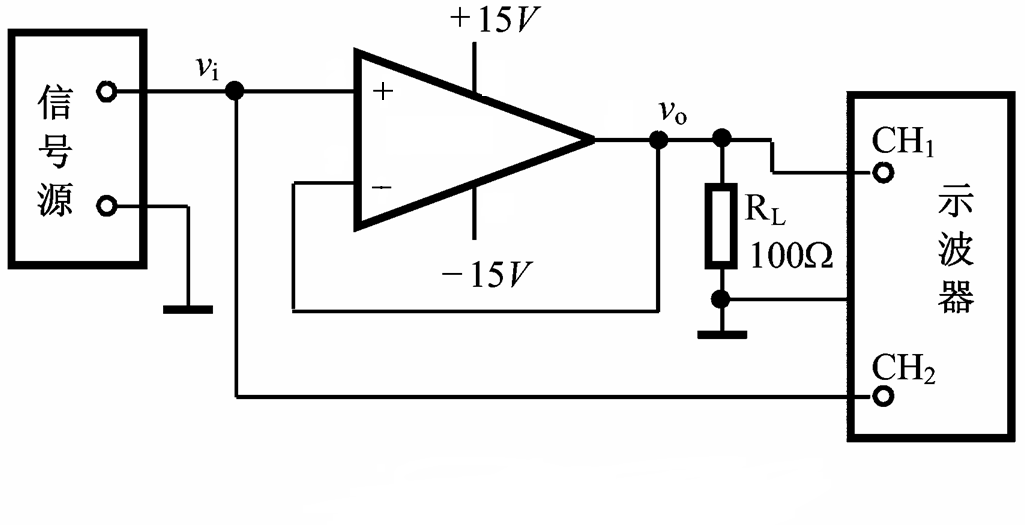
\includegraphics[width=1\textwidth]{通过电压跟随器连接}
		\caption{通过电压跟随器连接}
		\label{通过电压跟随器连接}
	\end{minipage}
\end{figure}

\subsection{反向比例加法电路}

(1)按照\reffig{加法器}在面包板上组装电路。电阻值取 $R_F=100 \mathrm{k}\Omega$, $R_1=10\mathrm{k}\Omega$, $R_2= 5.1\mathrm{k}\Omega$,安装电阻前先用万用表测试电阻值填入表中。

(2)按照\reffig{加法器}连接分压电路,其中$R_{s1}=R_{s2}=1\mathrm{k}\Omega$.将v1和v2连至图3-3对应输入端。


(3)检查无误后接通电源。从信号源送出频率为1kHz、峰-峰值为300mV 的正弦信号。用示波器测得$v_1$、$v_2$和$v_o$。 填入表中,并记录它们的波形。

(4)关闭电源,将$R_{s2}$改为$\mathrm{500}\Omega$,检查无误后接通电源,再次用示波器测得v1、v2和vo填入表中。

\begin{figure}[H]
	\centering
	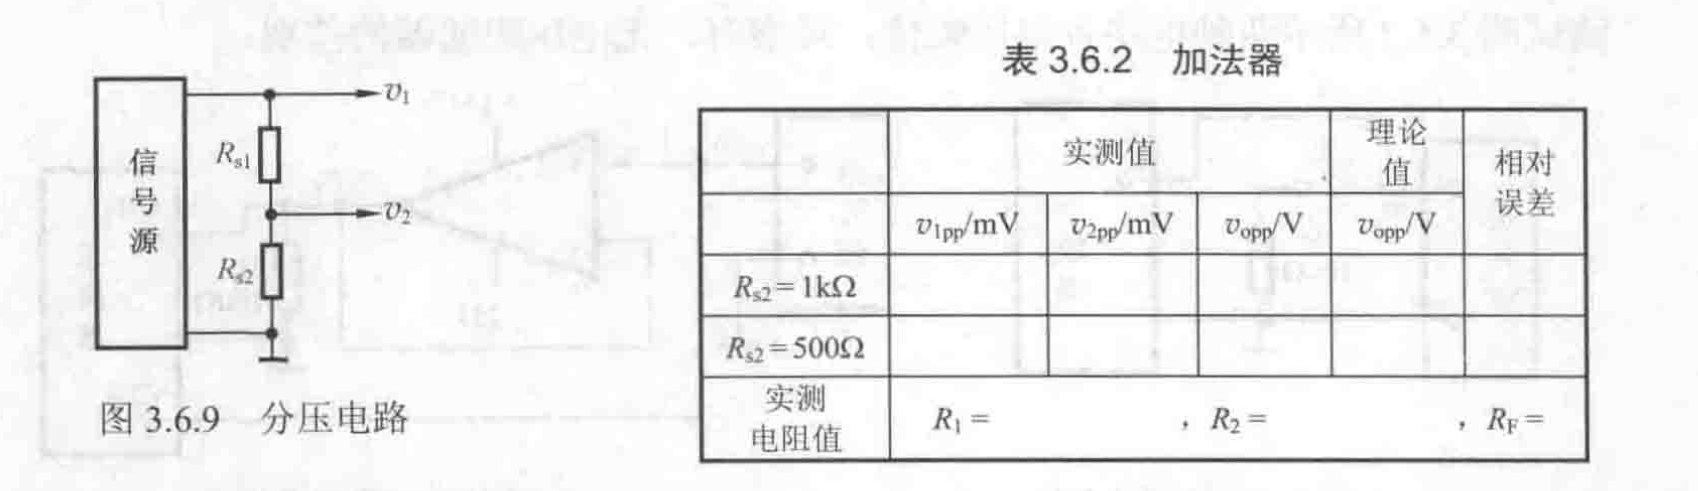
\includegraphics[width=1\textwidth]{加法器}
	\caption{加法器}
	\label{加法器}
\end{figure}


\subsection{积分电路}
按照\reffig{积分器}在面包板上组装电路。取$R_1=10\mathrm{k}\Omega$,\space $R_F=100\mathrm{k}\Omega$,$C=0.22\mathrm{μF}$,$R_P= 10\mathrm{k}\Omega$,输入f=200Hz,峰峰值为1V的正方波。用示波器测试$v_i$和$v_o$,并画出其波形。

\begin{figure}[H]
	\centering
	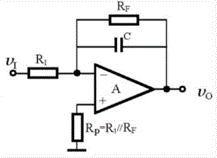
\includegraphics[width=0.5\textwidth]{积分器}
	\caption{积分器}
	\label{积分器}
\end{figure}

\clearpage

\section{实验原理}
\subsection{反向比例加法电路}
反向比例加法电路的实现如图4-1所示,输出电压的表达式为:
\begin{equation}
	v_{o}=-(\frac{R_{F}}{R_1}v_{i1}+\frac{R_{F}}{v_{i2}})
\end{equation}
$R_1, R_2, R_{F}$用于控制输出电压与输入电压的关系,可在运放的同相输入端加上一直流补偿电阻,其取值为 $R_1//R_2//R_{F}$, 减少输入失调电流对电路的影响。

\begin{figure}[H]
	\centering
	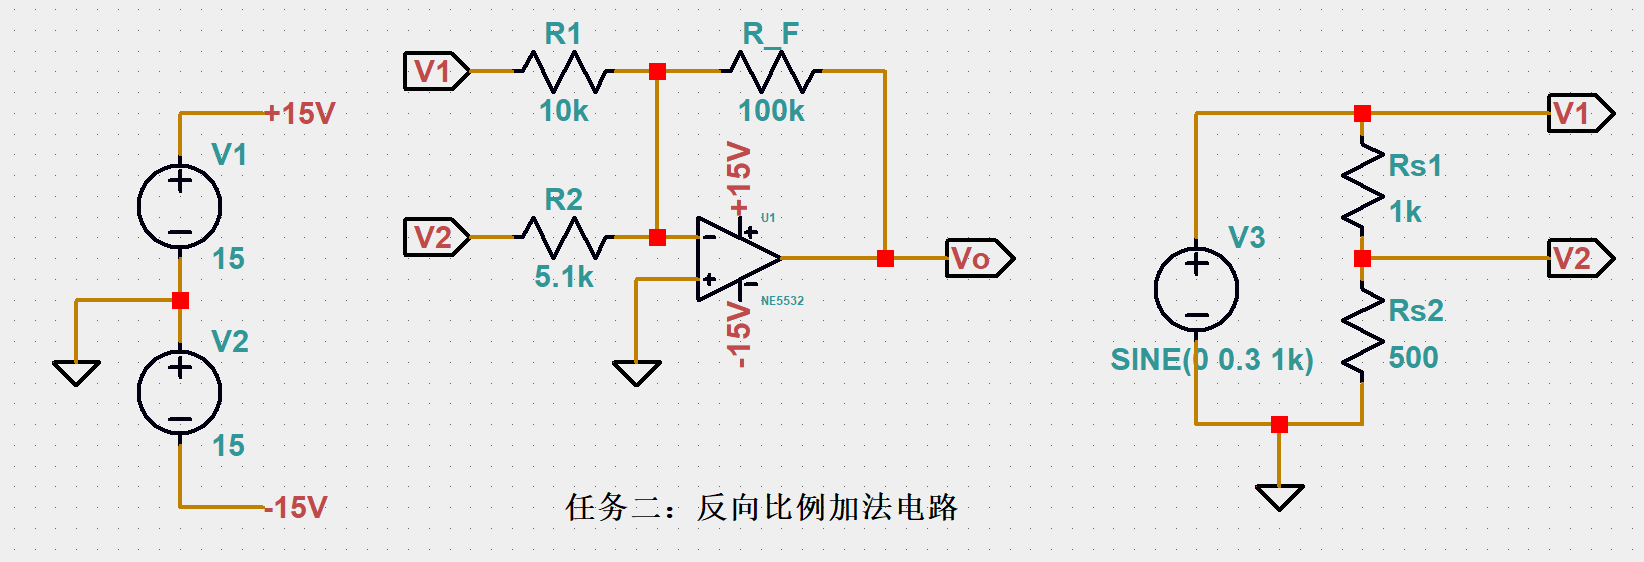
\includegraphics[width=1\textwidth]{反向比例加法电路}
	\caption{反向比例加法电路}
\end{figure}

\subsection{积分运算电路}
积分运算电路的电路图如\reffig{积分器}所示,当运算放大器开环电压增益足够大,且 $R_5$开路时,可认为 $i_{R}=i_{C}$,其中$i_R=\frac{V_i}{R_1}$, $i_c=-C \frac{dv_o(t)}{dt}$。设t=0时,电容器两端初始电压$v_o(O)$,则$v_o (t)=\int_{0}^{t} v_1(t) \mathrm{d}t+v_{o}(0)$。当 $v_o(0)=0$且输入信号$v_i(t)$为辐度为$V_i$的直流电压时,$v_o(t)=-\frac{1}{R_1C} \int_{0}^{t} V(t) \mathrm{d}t+v_o(0)=-\frac{1}{R_1C}V_it$,此时输出电压$v_o(t)$的波形是随时间线性下降的,当输入信号为正方波时,输出电压的稳态波形如图所示。

实际电路中,反馈电阻$\mathrm{R_f}$用于直流负反馈,目的是减小集成运算放大器输出端的直接漂移,且其阻值必须取得大一些,防止电路变成一阶低通滤波器。但同时$\mathrm{Rf}$的加入会对电容C产生分流作用,进而导致积分误差。因此,一般选用的元器件应满足 $R_{f}C \gg R_1C$,以减小误差。

\begin{figure}[H]
	\begin{minipage}[t]{0.5\linewidth}
		\centering
		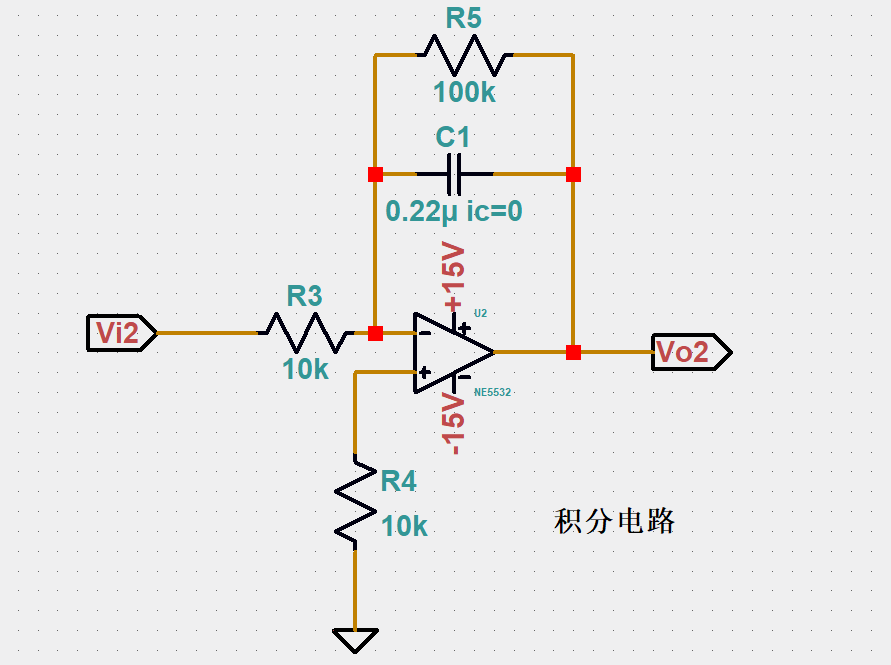
\includegraphics[width=1\textwidth]{积分电路}
		\caption{积分电路}
		\label{积分电路}
	\end{minipage}%
	\begin{minipage}[t]{0.5\linewidth}
		\centering
		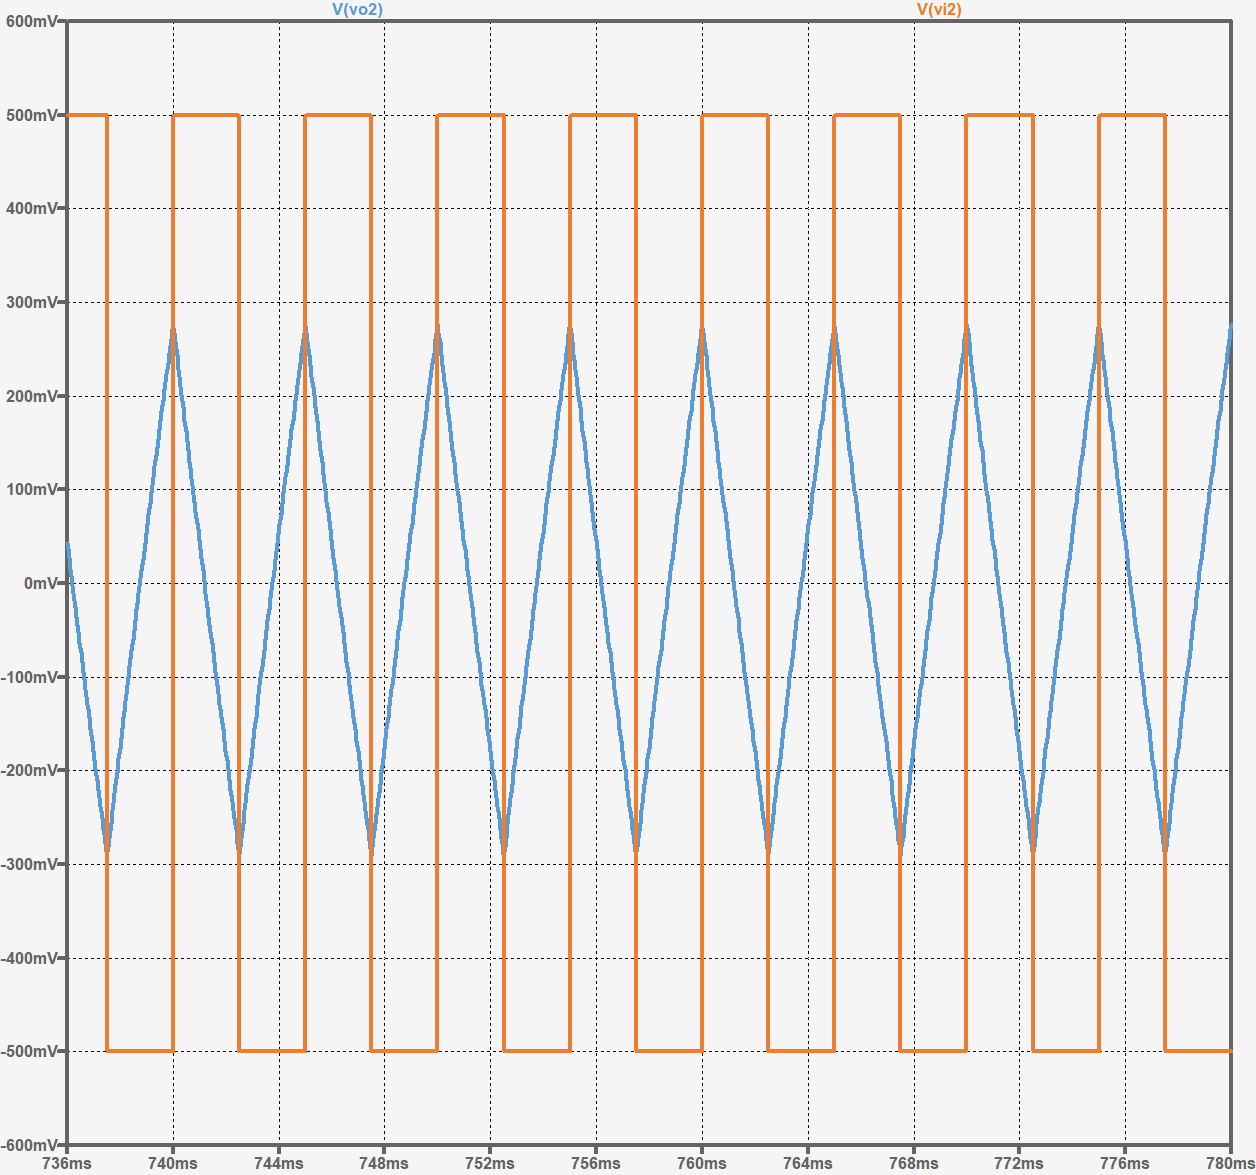
\includegraphics[width=1\textwidth]{积分电路波形}
		\caption{积分电路波形}
		\label{积分电路波形}
	\end{minipage}
\end{figure}


\section{实验过程}
按照上图连接电路,运放NE5532采用 $\pm \mathrm{12V}$双电源供电:

\subsection{电压跟随器实验}
按\reffig{直接连接}连接电路,分别测得不接 $R_L$和接入 $R_L$时的$v_i$和 $v_o$,填入\reftab{电压跟随器的作用}:

\begin{table}[H]
	\center
	\large
	\begin{tabular}{|c|cc|cc|c|}
		\hline
		\multirow{2}{*}{} & \multicolumn{2}{c|}{不接$R_L$}     & \multicolumn{2}{c|}{接入$R_L$} & \multirow{2}{*}{计算$R_s$/$\Omega$}                       \\ \cline{2-5}
		                  & \multicolumn{1}{c|}{$v_{ipp}$/V} & $v_{opp}$/V                  & \multicolumn{1}{c|}{$v_{ipp}$/V}  & $v_{opp}$/V &       \\ \hline
		无电压跟随器            & \multicolumn{1}{c|}{1.000}       & -                            & \multicolumn{1}{c|}{0.675}        & -           & 48.86 \\ \hline
		有电压跟随器            & \multicolumn{1}{c|}{1.020}       & 1.010                        & \multicolumn{1}{c|}{1.104}        & 1.010       & -     \\ \hline
	\end{tabular}
	\caption{电压跟随器的作用}
	\label{电压跟随器的作用}
\end{table}

\subsection{反向比例加法运算电路实验}
研究反向比例加法运算电路,在$v_i$端接入频率为1kHz、峰峰值为300mV的正弦波,直流偏置置零。示波器的两通道CH1、CH2分别接$v_1$、$v_2$和$v_1$、$v_o$,调节电位器以获取不同的测量电压值,记录测量数据\reftab{加法器}:

\begin{table}[H]
	\center
	\large
	\begin{tabular}{|c|ccccc|}
		\hline
		                                  & \multicolumn{3}{c|}{实测值}                                                                                & \multicolumn{1}{c|}{理论值} & \multirow{2}{*}{相对误差} \\ \cline{1-5}
		                                  &
		\multicolumn{1}{c|}{$v_{1pp}$/mV} &
		\multicolumn{1}{c|}{$v_{2pp}$/mV} &
		\multicolumn{1}{c|}{$v_{opp}$/V}  &
		\multicolumn{1}{c|}{$v_{opp}$/V}  &
		\\ \hline
		$R_{s1}=1\mathrm{k}\Omega$        &
		\multicolumn{1}{c|}{304.0}        &
		\multicolumn{1}{c|}{148.0}        &
		\multicolumn{1}{c|}{5.740}        &
		\multicolumn{1}{c|}{5.708}        &
		0.561\%                                                                                                                                                                                        \\ \hline
		$R_{s1}=500\Omega$                &
		\multicolumn{1}{c|}{304.0}        &
		\multicolumn{1}{c|}{106.0}        &
		\multicolumn{1}{c|}{4.800}        &
		\multicolumn{1}{c|}{4.851}        &
		1.051\%                                                                                                                                                                                        \\ \hline
		实测电阻值                             & \multicolumn{5}{c|}{$R_1=9.762\mathrm{k}\Omega,R_2=5.043 \mathrm{k}\Omega,R_F=98.792 \mathrm{k}\Omega$}                                                    \\ \hline
	\end{tabular}
	\caption{加法器}
	\label{加法器}
\end{table}
拍摄到的示波器波形图片如\reffig{加法电路——Rs1=500Ω}和\reffig{加法电路——Rs1=1KΩ}所示:

\begin{figure}[H]
	\centering
	\includegraphics[width=0.8\textwidth]{500欧}
	\caption{加法电路——Rs1=500Ω}
	\label{加法电路——Rs1=500Ω}
\end{figure}

\begin{figure}[H]
	\centering
	\includegraphics[width=0.8\textwidth]{1k欧}
	\caption{加法电路——Rs1=1KΩ}
	\label{加法电路——Rs1=1KΩ}
\end{figure}



\subsection{比例积分电路}
取$ R_1=10\mathrm{k}\Omega,R_F=100\mathrm{k}\Omega,C=0.22μF,R_P= 10\mathrm{k}\Omega$,$v_i$输入f=200Hz,峰峰值为1V的正方波。用示波器测试输入$v_i$和输出$v_o$,并画出其波形。

积分器波形如\reffig{积分器波形}所示,黄色表示 $v_i$,蓝色表示$v_o$。
\begin{figure}[H]
	\centering
	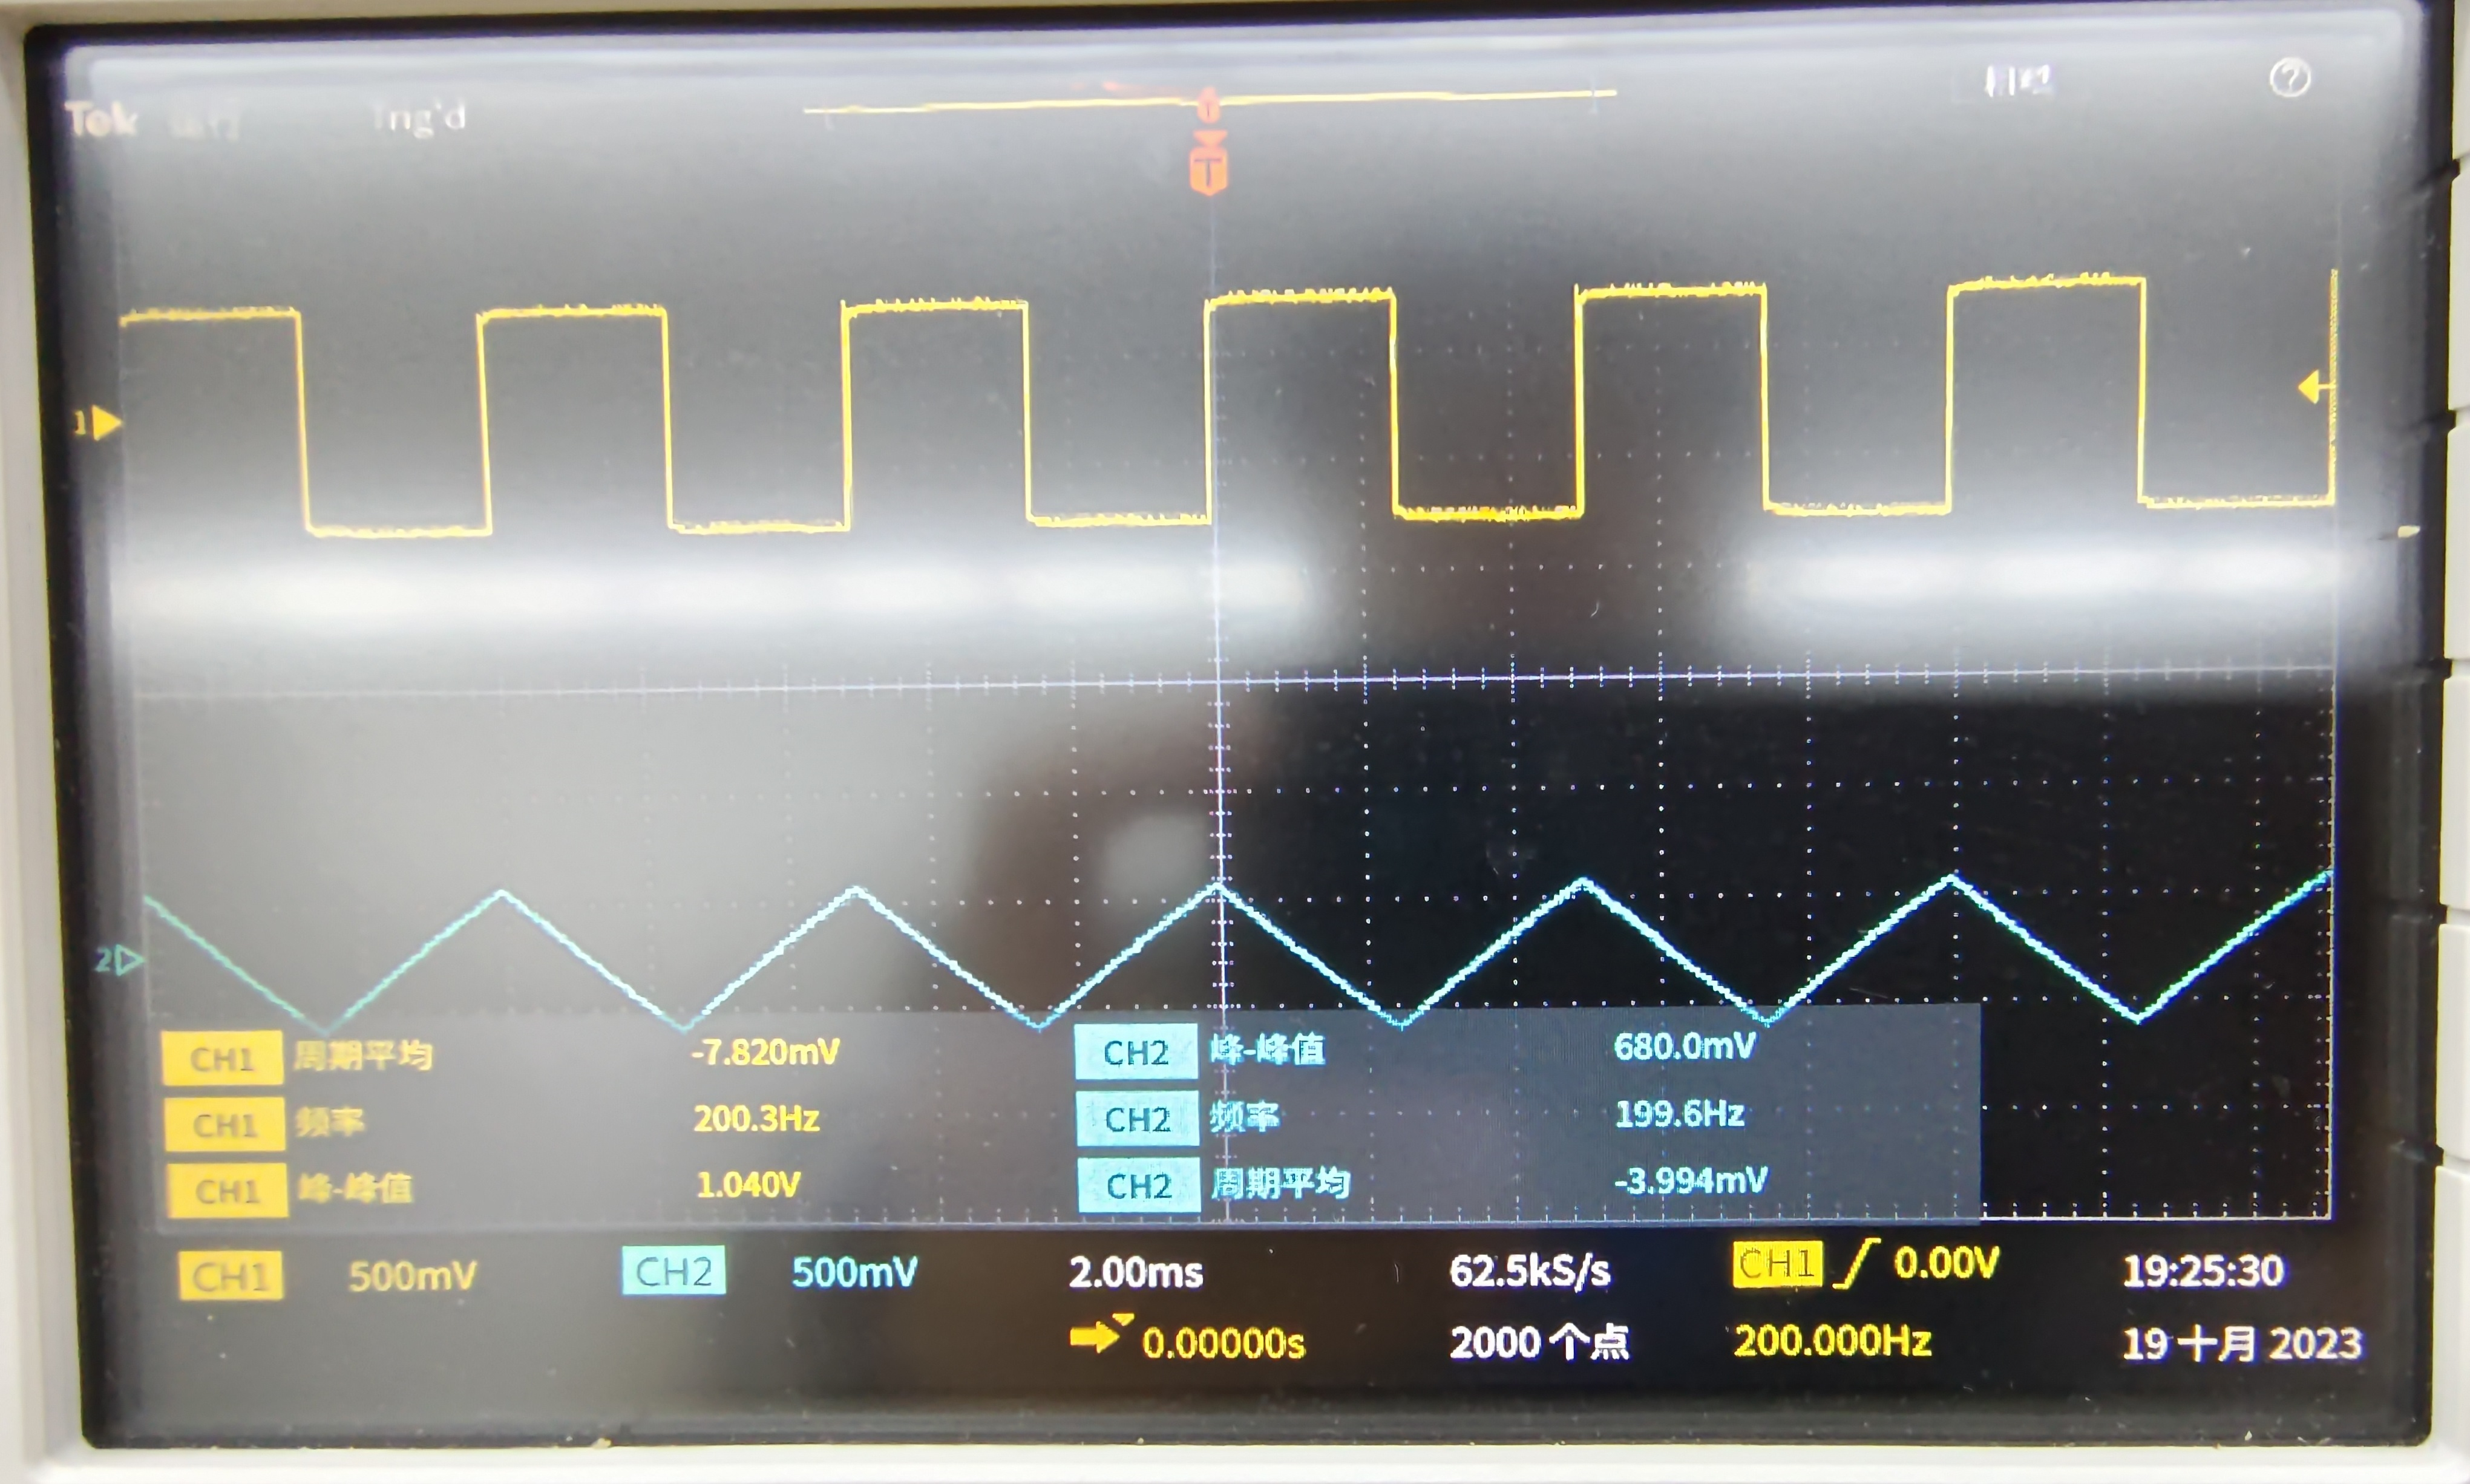
\includegraphics[width=1\textwidth]{积分器波形}
	\caption{积分器波形}
	\label{积分器波形}
\end{figure}

手绘波形:
\section{实验分析}
经分析,在反向比例加法运算电路实验中,实测值和理论值的误差均在2\%以内,误差较小,基本满足实验精度要求,电路正常工作,输出信号稳定光滑无毛刺,噪声较小。
\section{实验总结}

本次实验较为简单,涉及到的主要是基本运放电路的搭建和仪器的使用,通过本次实验的学习,我能够较为熟练的在面包板上搭建起简单的电路。我也认识到,通过搭建电路做实验能够加深自己对理论知识的理解。

与此同时,面包板的走线是一个难题,我的方法是尽量将元器件和跳线贴着面包板摆放,一来不容易松动,二来摆放工整,赏心悦目,同时方便检查。

% ------------------------------------ 附录 ------------------------------------ %
\clearpage
\appendix
\phantomsection


\end{document}
